% !TeX spellcheck = ru_RU
%pdflatex, utf8
\documentclass[unicode, 10pt, a5paper, oneside]{article}

% Установка полей страницы
%\usepackage{anysize}
%\marginsize{0.3cm}{0.3cm}{0.3cm}{0.3cm}
\usepackage[a5paper, margin=0.3cm, bindingoffset=0cm]{geometry}

% Поддержка русского языка
\usepackage[T2A]{fontenc}		% Корректная кодировка шрифта при использовании cm-super
\usepackage[utf8]{inputenc}		% Кодировка ввода
\usepackage[russian]{babel}		% Словарь расстановки переносов
%\usepackage{cmap}				% Перекодировка символов в pdf при использовании обычного cm

% Всякие математические фишки
\usepackage{amsmath}
\usepackage{amsfonts}
\usepackage{amssymb}

% Изменение цвета, работа с графикой
\usepackage{color}
\usepackage[pdftex]{graphicx}
\graphicspath{{images/}}

% Команда для вставки ссылок \url{URL}
\usepackage[hyphens]{url}
\urlstyle{rm}					% Стиль шрифта ссылок: с засечками

% Кликабельные ссылки внутри документа
\usepackage[unicode]{hyperref}

% Включает отступ у первого абзаца в разделе
\usepackage{indentfirst}

% Настрйока стиля списков
\usepackage{enumitem}
\setlist{noitemsep, leftmargin=*, labelindent=\parindent, topsep=0pt, parsep=0pt, partopsep=0pt}

\setlist[itemize,1]{label=$\diamond$}
\setlist[itemize,2]{label=\textendash}
\setlist[itemize,3]{label=$\star$}

\renewcommand{\alph}[1]{\asbuk{#1}} % Костыль для кирилической нумерации вместо латинской
\setlist[enumerate,1]{label=\arabic*)}
\setlist[enumerate,2]{label=\alph*)}
\setlist[enumerate,3]{label=(\arabic*)}


\usepackage{textcomp}			% Команды для вставки разных символов (градусы, проценты, итд)
\usepackage{float}				% Размещение плавающих объектов там где они созданы (X)
\usepackage{wrapfig}			% Обтекаемые текстом рисунки

% Подписи у флоатов
\setlength{\intextsep}{0pt} % Отстут вокруг плавающих окружений
\usepackage{caption}
\captionsetup{parskip=0pt}
\captionsetup[figure]{labelsep=period,justification=centering,singlelinecheck=false,textfont=small,labelfont=small,aboveskip=2pt,belowskip=0pt}

% Изменение формата заголовков разделов
\usepackage{titlesec}
\titleformat{\section}{\newpage\small\bfseries}{\thesection. }{0pt}{}{}
\titlespacing*{\section}{0pt}{0pt}{0pt}

\titleformat{\subsection}{\small\bfseries}{\thesubsection. }{0pt}{}{}
\titlespacing*{\subsection}{0pt}{0pt}{0pt}

\usepackage{array}				% Позволяет объявить свои типы колонок
\usepackage{calc}				% Математика, исп-ся для расчёта ширины колонки
\usepackage{longtable}			% Длинные таблицы

% Минимальный отступ в таблицах
\setlength{\tabcolsep}{1.5mm}

% Новые типы колонок. Ширина задётся как доля от linewidth
\newcolumntype{L}[1]{p{#1\linewidth-2\tabcolsep-2\arrayrulewidth}}
\newcolumntype{C}[1]{>{\centering}p{#1\linewidth-2\tabcolsep-2\arrayrulewidth}}
\newcolumntype{R}[1]{>{\raggedleft}p{#1\linewidth-2\tabcolsep-2\arrayrulewidth}}
\newcolumntype{U}[2]{p{#1\linewidth-(#2)}}

% Стараться не оставлять одиноких строк в начале и конце абзаца
\clubpenalty=1000
\widowpenalty=1000

% Расстановка отступов и переносов
\emergencystretch=2.5em			% Максимальный промежуток между словами
\tolerance=2000
\frenchspacing


\begin{document}

\setcounter{section}{80}

% Вопрос 81 -----------------------------------------------------------------
\section{Производственный и технологический процесс и их составляющие.}

Технология --- это совокупность способов, процессов обработки и оборудование, используемых при изготовлении элементов конструкции и сборке аппаратуры (механическое и электрическое соединение), обеспечивающих получение заданной конструкции (или заданной пространственной структуры) с высокой производительностью, малыми затратами и при минимальном вредном воздействии на окружающую среду или рабочего. Технология формируется на этапе проектирования ЭВС и реализуется на этапе производства.

В изготовлении ЭВС различают:

\begin{itemize}
\item производственный процесс
\item технологический процесс
\item технологические операции
\item переходы
\end{itemize}

Производственным процессом называется совокупность действий всего коллектива работающих, обеспечивающих превращение поступивших на предприятие материалов, полуфабрикатов в готовое изделие.

Производственный процесс  включает в себя:

\begin{itemize}
\item подготовку производства, получение, транспортирование, контроль и хранение материалов и комплектующих
\item технологические процессы изготовления деталей и сборки
\item изготовление технологической оснастки
\item обслуживание технологического и энергетического оборудования
\item управление технологическим процессом и производством
\item сбыт готовой продукции
\end{itemize}

Технологическим процессом называется часть производственного процесса, связанная с изготовлением, обработкой, сборкой, контролем изделия, т.е. с последовательной сменой состояния продукта производства (например, изготовление печатной платы).

Технологической операцией называется часть технологического процесса, представляющая совокупность производственных переходов и приемов, выполняемых непрерывно на одном рабочем месте одним рабочим (или группой рабочих) над определенной деталью или сборочной единицей (например, сверление отверстий в печатной плате, получение защитного рисунка, травление слоя фольги и т.д.).

Основными элементами технологических операций являются установ, технологический переход, вспомогательный переход, рабочий ход, вспомогательный ход и позиция.

Установ --- часть технологической операции, выполняемая при неизменном закреплении обрабатываемых заготовок или собираемой сборочной единицы.

Переход --- законченная часть технологической операции, выполняемая одними и теми же средствами технологического оснащения при постоянных технологических режимах и установке.

Вспомогательный переход --- законченная часть технологической операции, состоящая из действий человека и (или) оборудования, которые не сопровождаются изменением свойств предметов труда, но необходимы для выполнения технологического перехода. Например, закрепление заготовки, смена инструмента.

Рабочий ход --- законченная часть технологического перехода, состоящая из однократного перемещения инструмента относительно заготовки, сопровождаемого изменением формы, размеров и качества поверхности или свойств заготовки.

Вспомогательный ход --- законченная часть тех.перехода, состоящего из однократного перемещения инструмента относительно заготовки и необходимого для подготовки рабочего хода.

Позиция --- фиксированное положение, занимаемое неизменно закрепленной обрабатываемой заготовкой или собираемой сборочной единицей совместно с приспособлением относительно инструмента или неподвижной части оборудования для выполнения определенной части операции (обраб.в поворотном приспособлении).


% Вопрос 82 -----------------------------------------------------------------
\section{Исходные данные для разработки технологических процессов. Основные этапы разработки единичного технологического процесса.}

Исходными данными для разработки технологических процессов являются:

\begin{itemize}
\item конструкторская документация на изделие (сборочные чертежи, спецификации, рабочие чертежи, электрические схемы, перечни элементов, монтажные схемы и др.)
\item технические требования на изделие, где указываются дополнительные требования к изделию. Например, необходимость защиты, виды испытаний
\item объем выпуска продукции
\item сроки выпуска (еженедельно, ежемесячно, ежеквартально)
\item наличие технологического оборудования, оснастки
\item наличие освоенных типовых технологических процессов
\item справочная, нормативная литература, программы
\end{itemize}

Единичный технологический процесс (ТП) разрабатывается для изготовления или ремонта изделия одного наименования, типоразмера и исполнения независимо от типа производства.

Разработка единичного ТП включает в себя следующие этапы:

\begin{enumerate}
\item Анализ исходных данных и выбор действующего типового
технологического процесса или аналога единичного процесса
\item Выбор исходной заготовки и методов ее получения
\item Определение содержания операций, выбор технологических баз и составление технологического маршрута (последовательности обработки)
\item Выбор технологического оборудования, оснастки, средств автоматизации и механизации технологического процесса
\item Назначение и расчет режимов выполнения операций, нормирование переходов и операций технологического процесса, определение профессий и квалификации исполнителей, установление требований к технике безопасности
\item Расчет точности, производительности и экономической эффективности процесса
\item Оформление рабочей технологической документации (маршрутных и операционных карт, карт эскизов, ведомостей материалов, оборудования)
Необходимость каждого этапа, состава задач и последовательности решения устанавливается в зависимости от типа производства. Типизация технологических процессов позволяет устранить их многообразие с обоснованным сведением к ограниченному числу типов
\end{enumerate}


% Вопрос 83 -----------------------------------------------------------------
\section{Требования к оформлению технологической документации. Примеры записи технологических операций.}

Состав и правила оформления технологической документации определяются стандартами  единой системы технологической документации (ЕСТД). К технологическим относят графические и текстовые  документы, текстовые документы которые определяют технологический процесс изготовления или ремонта изделия и содержит необходимые данные для организации производства.

Состав документов зависит от стадии разработки технологического процесса, типа и характера производства. В условиях серийного и массового производства используются следующие документы по ГОСТ3.1102-81: Маршрутная карта (МК). Операционная карта (ОК). Карта эскизов (КЭ). Карта технологического процесса (КТП). Ведомость технологических документов (ВТД). Ведомость материалов (ВМ). Ведомость технологической оснастки (ВО). Комплектовочная карта (КК) и некоторые другие.

Маршрутная карта является основным технологическим документом, применяемым при разработке технологических процессов изготовления или ремонта изделия. Она  предназначена для маршрутного, маршрутно-операционного или операционного описания технологического процесса или указания полного состава технологических операций при операционным описании изготовления изделия, включая контроль и перемещения по всем операциям различных технологических методов в технологической последовательности с указанием данных об оборудовании технологической оснастке, материальных нормативах и трудовых затратах.

Карта технологического процесса предназначена для операционного описания технологического процесса изготовления изделия в технологической последовательности по всем операциям одного вида формообразования, обработки, сборки или ремонта с указанием переходов технологических режимов и данных о средствах технологического оснащения, материальных  и трудовых затратах.

Операционная карта содержит описание технологической операции с указанием переходов, режимов обработки и данных о средствах технологического оснащения. Она используется непосредственно  на рабочем месте.

Карта эскизов представляет собой графический документ, содержащий эскизы, схемы и таблицы и предназначены для пояснения выполнения технологического процесса, операций или перехода изготовления изделия и его составных частей, включая контроль и перемещения.

Основным технологическим документом является маршрутная карта,  при необходимости более подробного изложения операции используют операционные карты и карты техпроцесса.

Общие требования к технологическим документам изложены в ГОСТ 3.1104-82, правила оформления технологических документов --- в ГОСТ 3.1105-82, формы и правила оформления маршрутных карт --- в ГОСТ 3.1118-82, система обозначения технологических документов --- в ГОСТ 3.1201-82.

Обозначение документа строится по следующей структуре:

\begin{figure}[H]
\centering
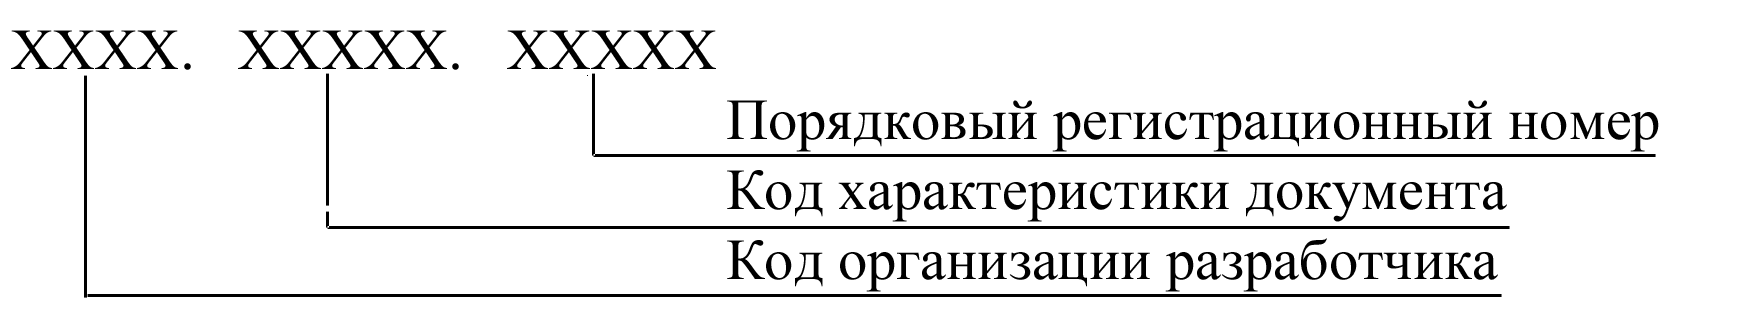
\includegraphics[width=0.6\textwidth]{83_code.png}
\caption{Структура кода документа}
\label{fig:83_code}
\end{figure}

В коде характеристики документа, состоящей из пяти цифр, первые два знака означают вид технологического документа, третья цифра --- вид техпроцесса по его организации, последние две цифры --- вид техпроцесса по его выполнению.

Виды технологического документа обозначаются следующим образом: 10 --- маршрутная карта, 20 --- карта эскизов, 30 --- комплектовочная карта, 42 --- ведомость оснастки, 43 ---  ведомость материалов, 50 --- карта технологического процесса.

Виды технологического процесса: 0 --- без указания; 1 --- единичный процесс; 2 --- типовой процесс, 3 --- групповой процесс.

Обозначение техпроцесса по методу выполнения: 01 --- технологический процесс изготовления изделия; 02 --- ремонт; 03 --- технический контроль; 40 --- механическая обработка; 60 --- изготовление деталей из пластмасс; 70 --- нанесение защитного и защитно-декоративного покрытия; 80 --- пайка; 88 --- слесарные, слесарно-сборочные и электромонтажные работы.

Таким образом, пример обозначения маршрутной карты технологического процесса электромонтажных работ с первым порядковым номером будет выглядеть следующим образом: КНФУ.10088.00001

При описании технологического процесса операции следует нумеровать числами ряда арифметической прогрессии, кратными пяти (5, 10, 15 и т.д.). Переходы следует нумеровать числам натурального ряда (1, 2, 3 и т.д.) Содержание операции (перехода) включает наименование метода  обработки, выраженного глаголом в повелительной форме (паять, установить, сверлить и т.д.), наименования обрабатываемой поверхности материала или детали,  Содержание операций и переходов должно быть сформулировано кратко, но с предельной ясностью и без возможности других толкований текста. Построение фразы или формулировки перехода должно обращать внимание исполнителя в первую очередь на главный предмет и действие, а затем указываются предметы и действия, посредством которых достигается основная цель. Например: «Установить транзистор поз. 17 на радиатор поз. 3 через прокладку поз.4 и закрепить винтом поз. 8 с шайбой поз.10»

При оформлении карты эскизов для сборочных операций должны быть изображены:

\begin{itemize}
\item базовая деталь или ее часть в положении, удобном для  работы
\item детали и узлы, устанавливаемые на данной операции, с указанием их схемных обозначений
\item выноски, указывающие позиции входящих деталей
\item контуры деталей, относительно которых размещаются провода, кабели, жгуты и навесные электрорадиоэлементы, монтируемые в данной операции
\end{itemize}

Изображения устанавливаемых деталей и узлов с их креплениями или монтируемых проводов должны выполняться линиями толщиной 0,6-0,8 мм, а остальные элементы показываются тонкими линиями (0,1 ---0,2 мм). На карте эскизов не показывают сборку деталей и узлов, выполненных предварительно.


% Вопрос 84 -----------------------------------------------------------------
\section{Основные методы изготовления печатных плат и их особенности.}

Методы изготовления печатных плат подразделяются на:

Субтрактивные, основанные на травлении фольгированного диэлектрика.

Аддитивные методы основаны на избирательном осаждении токопроводящего покрытия на диэлектрическое основание химическими или химико-гальваническими методами. При аддитивных методах толщина формируемого слоя меди составляет 15 --- 25 мкм, ширина проводников  0,10 --- 0,15 мм. Достоинствами методов являются  значительная экономия меди, снижение загрязнения окружающей среды, лучшая равномерность и однородность получаемых элементов печатного монтажа. Применение методов в массовом производстве печатных плат ограничено низкой производительностью процесса химической металлизации, интенсивным воздействием электролитов на диэлектрик.

Полуаддитивные, основанные на селективном осаждении проводящего покрытия химическими и гальваническими методами.

В зависимости от способа создания защитного рисунка химические методы подразделяются на сеточнохимический и фотохимический. Сеточнохимический метод основан на получении защитного рисунка при помощи специальной кислотостойкой краски, наносимой на поверхность печатной платы через сетчатый трафарет.

При фотохимическом методе защитный рисунок получают при помощи специального светочувствительного материала --- фоторезиста, наносимого на поверхность платы. В тех местах, где фоторезист был облучен через фотошаблон ультрафиолетовым светом, в результате фотополимеризации образуется защитная нерастворимая структура. Так как используемый при экспонировании фотошаблон является обратным по отношению к создаваемому слою проводников на печатной плате, метод получил название негативного. Разрешающая способность фотохимического метода примерно в два  раза выше, чем у сеточнохимического.

Комбинированные методы сочетают в себе химическое травление фольги исходного материала печатной платы и химическое осаждение и гальваническое  наращивание слоя меди в отверстиях и на поверхности проводников, т.е. методы пригодны для изготовления двухсторонних печатных плат.

В настоящее время находят применения  несколько иные методы создания печатных плат на основе тентинг-процесса и на основе метода ПАФОС (Получение Аддитивным Формированием Слоев).

Тентинг-метод. В двухсторонних слоях с межслойными переходами проводящий рисунок получают также путем травления медной фольги с гальваническим осажденным сплошным слоем меди по защитному рисунку схемы и с защитными завесками над металлизированными отверстиями в пленочном фоторезисте.

Односторонние ПП изготавливают субтрактивным химическим методом. Процесс изготовления не сложен, наименее трудоёмок и легко автоматизируется. Недостатком является эффект бокового подтравливания. Этого недостатка лишен аддитивный метод, основанный на избирательном осаждении химической меди на нефольгированный диэлектрик с нанесённым на поверхностный слой катализатором, инициирующим осаждение меди.

Двухсторонние ПП изготавливают позитивным комбинированным методом. Металлизацию отверстий производят электрохимическим методом, а проводящий рисунок получают травлением меди с пробельных мест. Такой метод обеспечивает хорошую адгезию элементов рисунка. Разрешающая способность ниже чем у химического метода. При полуаддитивном методе используется нефольгированный диэлектрик покрытый слоем полимерного материала. Малое боковое подтравливание и лучшая адгезия дают возможность получить высокую разрешающую способность.

Методы изготовления МПП по получению межслойных соединений делятся на 2 группы:

\begin{enumerate}
\item Методы на основе химико-гальванических процессов (метод металлизации сквозных отверсти, метод попарного прессования, метод послойного нарашивания)
\item Методы, в которых межслойные соединения осуществляются посредством пайки, сварки и добавочных элементов (метод открытых контактных, площадок, метод выступающих выводов)
\end{enumerate}


% Вопрос 85 -----------------------------------------------------------------
\section{Конструктивно-технологические разновидности радиоэлектронных узлов и их сопоставительный анализ.}

Проанализируем представленные в таблице конструкции радиоэлектронных узлов и технологические особенности их изготовления.

Методами монтажа на поверхность изготавливают узлы исполнения 1 и 2. Несмотря на явные преимущества с точки зрения улучшения массогобаритных показателей данные конструкции недостаточно распространены из-за ряда ограничений по номенклатуре элементной базы (по мощности, величинам емкости электролитических конденсаторов, ограниченности типов активных компонентов и т.д.).

В узлах конструктивного исполнения 1 применяют только КМП, которые устанавливают с одной стороны печатной платы (КМП1).

\begin{figure}[H]
\centering
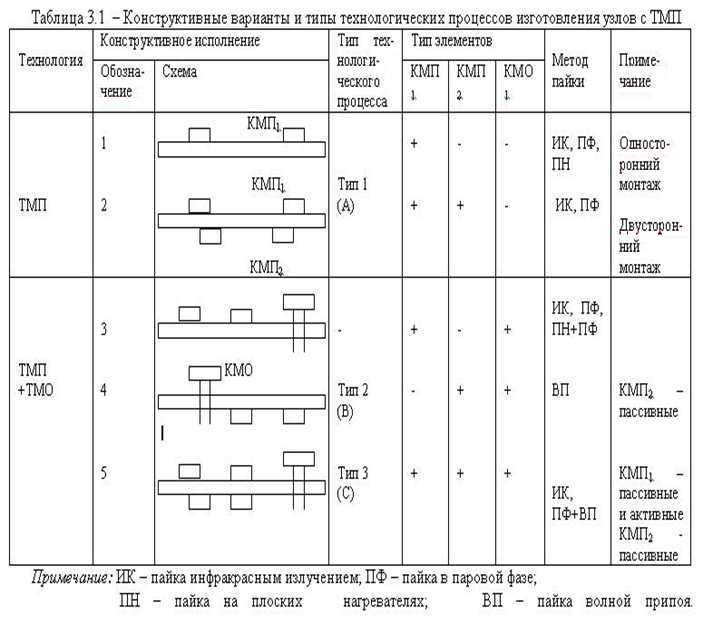
\includegraphics[width=0.8\textwidth]{85_types.png}
\caption{Типы монтажа}
\label{fig:85_types}
\end{figure}

Монтаж компонентов для данного исполнения состоит из следующих операций:

\begin{itemize}
\item нанесение припойной пасты через трафареты на контактные площадки печатной платы
\item установка компонентов на контактные площадки
\item оплавление припойной пасты
\item промывка печатной платы от остатков флюса
\item контроль паяных соединений
\item устранение непропаев,  закорачиваний
\item Возможно также для данного исполнения использования пайки волной припоя по следующей схеме
\begin{figure}[H]
\centering
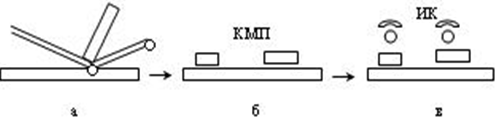
\includegraphics[width=0.5\textwidth]{85_scheme.png}
\caption{Схема технологического процесса монтажа исполнения 1 (процесс типа I): а --- нанесение паяльной пасты;  б --- установка КМП;  в --- оплавление пасты}
\label{fig:85_scheme}
\end{figure}
\item нанесение клея на поверхность платы между контактными площадками
\item установка КМП на контактные площадки
\item полимеризация клея под воздействием ультрафиолетового или инфракрасного излучения (в зависимости от типа используемого клея)
\item поворот платы на 180 \textcelsius
\item пайка волной припоя
\end{itemize}

Недостатком данного варианта технологического процесса является необходимость применения только компонентов, устойчивых к действию расплавленного припоя   (обычно это простые чип-компоненты типа резисторов и конденсаторов), а также введение дополнительных операций по нанесению клея и его полимеризации.

Исполнение 2 обеспечивает  наивысшую плотность компоновки печатных плат.

Изготовление проводят методами ТМП по следующей схеме:

\begin{itemize}
\item на контактные площадки обратной стороны печатной платы наносят через трафарет припойную пасту;
\item под компонент наносят микрокаплю клея (для компонентов простой формы и малых размеров данная операция может быть исключена, так как компонент способен удерживаться на плате при ее переворачивании за счет сил поверхностного натяжения);
\item производят установку  КМП1; 
\item осуществляют полимеризацию клея УФ или ИК излучением;
\item производят оплавление пасты припоя путем пайки в паровой фазе, инфракрасным нагревом,  нагревом на плоских нагревателях, лазерным или световым лучом;
\item плату переворачивают и наносят пасту припоя на вторую сторону;
\item устанавливают компоненты КМП2;
\item проводят оплавление пасты припоя;
\item осуществляют промывку узла и его контроль.
\end{itemize}

При такой последовательности операций пайка осуществляется ИК излучением с односторонним нагревом.

При пайке в паровой фазе (ПФ), а также ИК излучением с верхним и нижним расположением излучателей операцию оплавления пасты после установки КМП1 не проводят, выполняя в этом случае пайку одновременно с двух сторон.

Конструктивное исполнение 3, 4 и 5 применяют при отсутствии ряда компонентов, предназначенных для поверхностного монтажа.

Радиоэлектронные узлы конструктивного исполнения  3 собирают по следующей схеме:

\begin{itemize}
\item наносят на контактные площадки для КМП припойную пасту;
\item устанавливают КМП1;
\item производят оплавление припойной пасты;
\item устанавливают в отверстия КМО1;
\item осуществляют пайку КМО1 волной припоя;
\item выполняют промывку узла и его контроль.
\end{itemize}

Конструктивное исполнение 4 включает КМП на нижней стороне платы, а КМО --- на верхней стороне.

Сборку и монтаж проводят в следующей последовательности:

\begin{itemize}
\item на поверхность платы наносят дозатором клей;
\item устанавливают КМП1;
\item выполняют полимеризацию клея УФ или ИК излучением;
\item переворачивают плату и устанавливают КМО2; 
\item выполняют одновременную пайку КМП1 и КМО2 волной припоя
\item промывают сборку и осуществляют контроль.
\end{itemize}

При пайке многовыводных КМП могут возникнуть трудности, связанные с непропаем в результате теневого эффекта или же с появлением закорачиваний выводов компонента. Для предотвращения появления таких дефектов применяют пайку двойной волной припоя.

\begin{figure}[H]
\centering
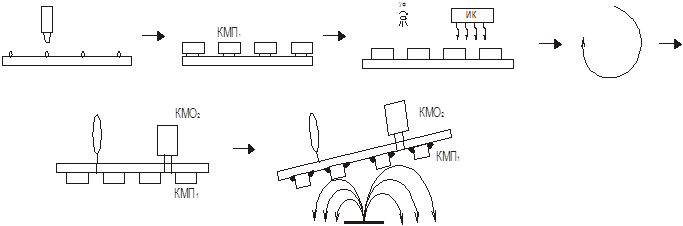
\includegraphics[width=1.0\textwidth]{85_double.png}
\caption{Вариант двухстороннего монтажа}
\label{fig:85_double}
\end{figure}

% Вопрос 86 -----------------------------------------------------------------
\section{Основные технологические операции при изготовлении радиоэлектронных узлов с монтажом на поверхность.}

Технология сборки узлов с монтажом на поверхность имеет ряд особенностей.
\begin{enumerate}
\item Перед выполнением пайки компоненты должны быть зафиксированы на плате. Такое закрепление может быть получено при помощи паяльной пасты, наносимой на контактные площадки перед монтажом компонента, либо при помощи микрокапли клея, на которую ставится компонент.
\item Технология монтажа на поверхность в чистом виде применяется сравнительно редко. Обычно на печатную плату одновременно устанавливаются и КМП, и КМО. В результате используется 5 конструктивно-технологических разновидностей узлов с применением ТМП.
\item Миниатюрность компонентов, отсутствие на многих из них маркировки предполагают только автоматизированный монтаж и пайку.
\item Существенное уменьшение как геометрических размеров компонентов, так и увеличение плотности расположения выводов и печатных проводников создает серьезные технологические трудности как в части уменьшения всех погрешностей при изготовлении печатных плат, так и при установке компонентов с высокой точностью позиционирования, обеспечения надежности процесса пайки (недопустимости закорачивания выводов и проводников при малом расстоянии между ними, изменения положения компонентов при пайке в результате действия сил поверхностного натяжения), согласованности температурных коэффициентов термического расширения  компонентов и оснований печатных плат.
\end{enumerate}

Монтаж компонентов для данного исполнения состоит из следующих операций:
\begin{itemize}
\item нанесение припойной пасты через трафареты на контактные площадки печатной платы
\item установка компонентов на контактные площадки
\item оплавление припойной пасты
\item промывка печатной платы от остатков флюса
\item контроль паяных соединений
\item устранение непропаев,  закорачиваний
\item возможно также для данного исполнения использования пайки волной припоя
\item нанесение клея на поверхность платы между контактными площадками
\item установка КМП на контактные площадки
\item полимеризация клея под воздействием ультрафиолетового или инфракрасного излучения (в зависимости от типа используемого клея)
\item поворот платы на 180 \textcelsius
\item пайка волной припоя
\end{itemize}

\begin{figure}[H]
\centering
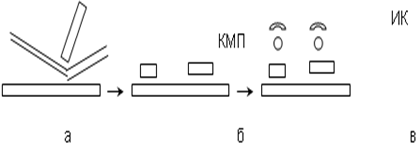
\includegraphics[width=0.5\textwidth]{86_scheme.png}
\caption{Схема технологического процесса монтажа исполнения 1 (процесс типа I): а --- нанесение паяльной пасты;  б --- установка КМП;  в --- оплавление пасты}
\label{fig:86_scheme}
\end{figure}

Исполнение 2 обеспечивает  наивысшую плотность компоновки печатных плат.

Изготовление проводят методами ТМП по следующей схеме:

\begin{figure}[H]
\centering
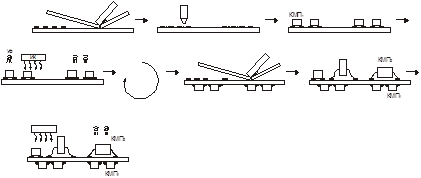
\includegraphics[width=0.5\textwidth]{86_scheme2.png}
\caption{Изготовление по схеме ТМП}
\label{fig:86_scheme2}
\end{figure}

\begin{itemize}
\item на контактные площадки обратной стороны печатной платы наносят через трафарет припойную пасту;
\item под компонент наносят микрокаплю клея (для компонентов простой формы и малых размеров данная операция может быть исключена, так как компонент способен удерживаться на плате при ее переворачивании за счет сил поверхностного натяжения);
\item производят установку  КМП1; 
\item осуществляют полимеризацию клея УФ или ИК излучением;
\item производят оплавление пасты припоя путем пайки в паровой фазе, инфракрасным нагревом,  нагревом на плоских нагревателях, лазерным или световым лучом;
\item плату переворачивают и наносят пасту припоя на вторую сторону;
\item устанавливают компоненты КМП2;
\item проводят оплавление пасты припоя;
\item осуществляют промывку узла и его контроль.
\end{itemize}

При такой последовательности операций пайка осуществляется ИК излучением с односторонним нагревом.

При пайке в паровой фазе (ПФ), а также ИК излучением с верхним и нижним расположением излучателей операцию оплавления пасты после установки КМП1 не проводят, выполняя в этом случае пайку одновременно с двух сторон.


% Вопрос 87 -----------------------------------------------------------------
\section{Нанесение паяльной пасты и клея и используемое при этом оборудование.}

Применяются два основных способа нанесения. Метод дозирования с применением пневматических дозаторов хорош тем, что он не привязан к трафарету, и оператор может работать с любой платой. Таким дозатором удобно пользоваться при большом количестве различных типов плат или на опытном участке, где при разработке плата меняется несколько раз. Слабая сторона этого метода в его низкой производительности, которая определяется мастерством оператора.

Второй метод --- метод трафаретной печати, является групповым. Он основан на продавливании паяльной пасты  через сетчатый или металлический трафарет. Для этого применяются устройства трафаретной печати различного уровня сложности и производительности.

Метод дозирования с применением пневматических дозаторов хорош тем, что он не привязан к трафарету, и оператор может работать с любой платой. Таким дозатором удобно пользоваться при большом количестве различных типов плат или на опытном участке, где при разработке плата меняется несколько раз. Слабая сторона этого метода в его низкой производительности, которая определяется мастерством оператора.

Для работы в сборочных линиях  разработана широкая гамма оборудования, обеспечивающего нанесение от 1500 до 140000 доз в час с точностью позиционирования в 50 мкм. Высокая точность позиционирования достигается использованием системы технического зрения, осуществляющей автоматическую коррекцию по реперным знакам, и прецизионных высокоскоростных приводов по осям X, Y и Z. Наиболее совершенными приводами на сегодняшний день считаются шарико-винтовые пары (ШВП), работающие независимо или совместно.

Вращение ШВП в одинаковом направлении приводит к перемещению привода по оси Y, а вращение в противоположных направлениях  --- к перемещению привода по оси Х.

Автоматы трафаретной печати имеют, как правило, компьютерное управление в сочетании с программированием в среде Windows NT, что делает их удобными в управлении и позволяет оператору быстро обучаться. Наиболее совершенные автоматы трафаретной печати типа HORIZON и INFININY имеют время полного цикла 12,5 и 8 секунд, обеспечивают гибкое управление процессом нанесения паяльной пасты, имеют систему контроля загрязнения окон трафарета с автоматическим включением очистки трафарета.

\begin{figure}[H]
\centering
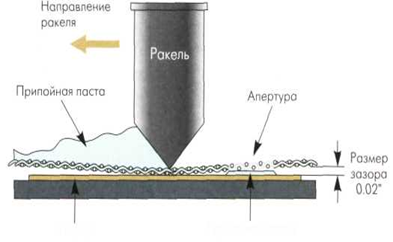
\includegraphics[width=0.5\textwidth]{87_tprint.png}
\caption{Схема процесса нанесения клея через трафарет}
\label{fig:87_tprint}
\end{figure}


% Вопрос 88 -----------------------------------------------------------------
\section{Принципы организации работы сборочных автоматов.}

По производительности, т.е. по количеству устанавливаемых на плату компонентов в единицу времени автоматы подразделяют на машины малой (до 1 тыс/час), средней (до 10 тыс/ч) и высокой (свыше 10 тыс/час) производительности.

В зависимости от способа установки различают линейные автоматы, автоматы последовательного, параллельного и последовательно-параллельного типов. Цикл работы любого сборочного автомата включает в себя следующие операции: выбор из магазина (накопителя) компонента конкретного типа и номинала, перемещение его к печатной плате, установка на печатную плату с заданной точностью.

В состав автомата сборки обычно входят следующие типовые блоки: накопитель (магазин с компонентами), монтажная головка или блок головок с захватами, двухкоординатный стол, устройство позиционирования, оптическая система контроля положения и обнаружения пропущенных компонентов, устройство контроля электрических параметров чип-компонентов, система управления на базе микроконтроллеров или микроЭВМ.

\begin{itemize}
\item элементы для поверхностного монтажа поставляются
\item на пластиковых лентах, смотанных в бобины
\item в трубчатых магазинах (кассетах)
\item россыпью
\end{itemize}

Наибольшее распространение получила подача элементов с бобины, а также из кассеты.

Монтажные головки осуществляют захват компонентов при помощи миниатюрных вакуумных присосок, что существенно снизило риск повреждения компонента по сравнению с механическими захватами.

Двухкоординатный стол перемещается на воздушной подушке под действием линейных двигателей. Стол должен обладать высоким быстродействием и высокой точностью позиционирования. Наилучшими характеристиками на сегодняшний день в этом отношении имеют приводы на основе шарико-винтовой пары.

Система позиционирования основана на использовании технического зрения  для контроля положения платы перед монтажом и корректировки положения устанавливаемого компонента. Контроль осуществляется посредством реперных знаков. Некоторые системы способны также контролировать состояние выводов сложных компонентов (их наличие, отсутствие повреждений).

Сборочные автоматы должны обладать несколькими степенями свободы: обеспечивать взаимное перемещение монтажной головки, печатной платы и накопителя в трех направлениях, обеспечивать разворот монтируемого компонента  на угол 90 или 45\textdegree (для компонентов в корпусах типа QFP и PLCC). Конструктивная реализация перемещения стола с печатной платой в вертикальном направлении (вдоль оси z), а также поворот ее вокруг этой оси (угол $\theta$) достаточна сложна и приводит к снижению быстродействия.

В ряде случаев вместо линейного перемещения накопителя используют поворот кассет с элементами, т.е. применяют карусельную конструкцию. Используют также блок монтажных головок, которые последовательно перемещаются  из одной рабочей позиции в другую (револьверная головка с несколькими захватами). Блок монтажных головок позволяет производить выборку нужного компонента из соответствующего магазина, а также осуществлять контроль электрических параметров и позиционирования компонента. Автомат имеет револьверную головку с четырьмя захватами и четырьмя рабочими позициями через 90\textdegree.

Упакованные в ленту компоненты размещают на бобинах, которые устанавливают в карусель, поворачивающуюся вокруг вертикальной оси. Печатную плату располагают на двухкоординатном столе. При работе автомата нужный компонент подается в питатель за счет поворота карусели.

Вакуумный захват забирает компонент, револьверная головка поворачивает его на 90\textdegree. Компонент передается в устройство контроля электрических параметров. В следующей позиции КМП центрируется, т.е. его положение корректируется по отношению к установочному месту на плате. Затем головка поворачивается в следующую позицию, плата с помощью стола перемещается в рабочее положение и происходит установка компонента на плату, после чего цикл повторяется.

\begin{figure}[H]
\centering
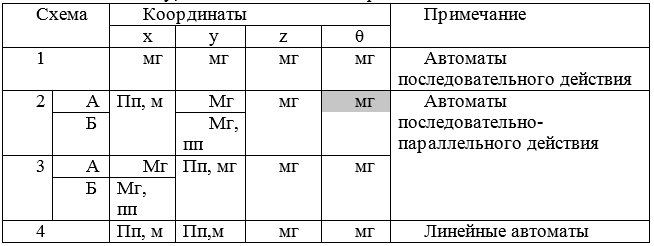
\includegraphics[width=0.65\textwidth]{88_table.png}
\caption{МГ --- монтажная головка, ПП --- печатная плата; М --- магазин с компонентами.}
\label{fig:88_table}
\end{figure}


% Вопрос 89 -----------------------------------------------------------------
\section{Особенности выполнения пайки при изготовлении электронных модулей (пайка оплавлением, волной припоя, селективная пайка).}

\subsection*{Пайка оплавлением}

Пайка оплавлением припойной пасты применима только к технологии поверхностного монтажа печатных плат. В основном все существующие системы пайки оплавлением ориентированы на ИК нагрев, однако ранее использовались системы с "темными" нагревателями. Сегодня нагрев такие нагреватели используются как вспомогательные: прогрев платы на предварительных этапай пайки с целью избежания тепловых поводок. При этом необходимо учесть, что передача тепла излучением в ИК области требует прозрачности корпусов электронных компонентов (в случае подкорпусного расположения выводов). Большинство современных SMD компонентов удовлетворяют этому требованию.

Процесс пайки компонентов, собранных на плате, с помощью ИК нагрева аналогичен пайке в ПГФ, за исключением того, что нагрев платы с компонентами производится не парами жидкости, а ИК излучением.

Основным механизмом передачи тепла, используемым в установках пайки с ИК нагревом, является излучение. Передача тепла излучением имеет большое преимущество перед теплопередачей за счет теплопроводности и конвекции, так как это единственный из механизмов теплопередачи, обеспечивающий передачу тепловой энергии по всему объему монтируемого устройства. Остальные механизмы теплопередачи обеспечивают передачу тепловой энергии только поверхности монтируемого изделия. В отличие от пайки в ПГФ, в процессе пайки с ИК-излучением скорость нагрева регулируется изменением мощности каждого излучателя и скорости движения транспортера с платами. Поэтому термические напряжения в компонентах и платах могут быть снижены посредством постепенного нагрева микросборок. Основным недостатком пайки с ИК нагревом является то, что количество энергии излучения, поглощаемой компонентами и платами, зависит от поглощающей способности материалов, из которых они изготовлены. Поэтому нагрев осуществляется неравномерно в пределах монтируемого 
устройства. Пайка кристаллоносителей без выводов или с J-образными выводами может оказаться невозможной в установках с ИК-нагревом, если компонент непрозрачен для ИК-излучения.

В некоторых установках для пайки с ИК-нагревом вместо ламп ИК-излучения применяются панельные излучающие системы. В этом случае излучение имеет большую длину волны, чем излучение традиционных источников. Излучение такой системы не нагревает непосредственно микросборку, а поглощается технологической средой, которая в свою очередь передает тепло микросборке за счет конвекции. Этот способ пайки устраняет ряд недостатков, присущих традиционной пайке с ИК нагревом, таких, как неравномерный прогрев отдельных частей микросборки и невозможность пайки компонентов в корпусах, непрозрачных для ИК-излучения. Панельные излучатели имеют ограниченный срок службы и обеспечивают намного меньшую скорость нагрева, чем традиционные источники ИК излучения. Однако при их использовании может не потребоваться технологическая среда из инертного газа.

\subsection*{Пайка волной припоя}

Она применяется для пайки компонентов в отверстиях плат (традиционная технология DIP-монтажа). С ее помощью можно производить пайку поверхностно-монтируемых компонентов с несложной конструкцией корпусов, устанавливаемых на одной из сторон коммутационной платы.

Пайка осуществляется следующим образом. Платы, установленные на транспортере, проходят зону предварительного нагрева, что исключает тепловой удар на этапе пайки. Затем плата проходит над волной припоя. Сама волна, ее форма и динамические характеристики являются наиболее важными параметрами оборудования для пайки. Изменяя характеристики сопла, можно менять форму волны. В наиболее простых установках для пайки применяется симметричная волна, однако лучшее качество пайки получается при использовании несимметричной формы волны (в виде греческой буквы «омега», Z-образную, Т-образную и др.). Направление и скорость движения потока припоя, достигающего платы, также могут варьироваться, но они должны быть одинаковы по всей ширине волны. Угол наклона транспортера для плат тоже регулируется. Некоторые установки для пайки оборудуются дешунтирующим воздушным «ножом», который обеспечивает уменьшение количества перемычек припоя. «Нож» располагается сразу же за участком прохождения волны припоя и включается в работу, когда 
припой находится еще в расплавленном состоянии на коммутационной плате. Узкий поток нагретого воздуха, движущийся с высокой скоростью, уносит с собой излишки припоя, тем самым разрушая перемычки и способствуя удалению остатков припоя.

\subsection*{Селективная пайка}

Системы селективной пайки миниволной припоя отличаются от обычных систем пайки одинарной или двойной волной припоя тем, что в установках пайки второго типа происходит групповая пайка компонентов, то есть вся плата проходит через волну припоя. Система селективной пайки паяет соединения выборочно, в соответствии с заданной программой. Это происходит следующим образом: в машину загружается рабочая программа, печатная плата устанавливается в паллету, и запускается программа пайки. Транспортная система установки доставляет паллету с платой к модулю спрей-флюсования, который наносит дозы флюса на заданные точки, и к модулю предварительного нагрева. Затем паллета перемещается к паяльной насадке, где происходит пайка соединений в соответствии с заданной программой. Паллета с платой опускается к паяльной насадке и погружает выводы паяемых компонентов в миниволну припоя. Пайка может быть точечной --- отдельных выводов компонентов, и линией --- ряда выводов компонента. После выполнения программы пайки готовая плата 
возвращается в окно загрузки.

Кроме того, избирательная пайка может осуществляться точечным нагревом, например, лазерным лучом.


% Вопрос 90 -----------------------------------------------------------------
\section{Особенности выполнения ремонтных работ: демонтаж и монтаж компонентов.}

Ручная пайка может применяться в случае выполнения необходимых ремонтных работ, установке отдельных видов КМО и КМП, при отладке конструкций узлов и при малой программе выпуска изделий.  Для этих целей выпускается широкая гамма инструмента и оборудования, известных как паяльные станции. По сравнению с типичным паяльником подобные станции позволяют весьма точно выдерживать температуру пайки благодаря наличию термодатчиков и микропроцессорной системы управления, имеют широкий набор насадок для распайки  и демонтажа различных корпусов. Наиболее совершенные паяльные станции обеспечивают также дозированную подачу паяльной пасты или клея, вакуумный отсос избытка припоя.

При ручной пайке обычным паяльником продолжительность операции определяется радиомонтажником, а обеспечение стабильности температуры --- используемым инструментом. При этом температура жала паяльника при выполнении серии паек существенно изменяется.

\begin{figure}[H]
\centering
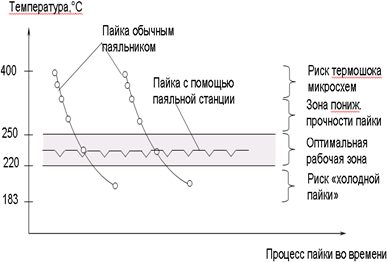
\includegraphics[width=0.65\textwidth]{90_soldering.png}
\caption{Изменение температуры жала в процессе пайки}
\label{fig:90_soldering}
\end{figure}

Перед началом пайки серии соединений температура его жала может находиться далеко за верхним пределом оптимальной рабочей зоны и достигать значения 350 --- 400 \textcelsius, а после нескольких операций за короткий промежуток времени она опускается ниже оптимальной рабочей зоны. Время пайки постепенно увеличивается, а температура может снизиться вплоть до области холодной пайки.

Холодная пайка имеет место при температурах выше 183 \textcelsius, но ниже 220 \textcelsius, когда припой уже расплавился, но диффузия металлов с образованием достаточно интерметаллического слоя еще не произошла. Прочность такого соединения очень низка.

С другой стороны, завышенная температура пайки или избыточное время нахождения припоя в расплавленном состоянии тоже чреваты снижением прочности соединения. Причина заключается в том, что в результате химической реакции между медью и оловом образуется диффузионный слой Cu3Sn / Cu6Sn5, называемый иногда как  интерметаллический  компаунд. Именно этот слой взаимопроникновения металлов выполняет роль механической связки в паяном соединении. Исследования показывают, что максимальная прочность паяного соединения имеет место при толщине данного слоя 0,5 мкм. При меньшей толщине слоя пайка является холодной, при большей --- ухудшаются характеристики эластичности слоя, тогда как именно это свойство позволяет компенсировать напряжения, возникающие в паяном соединении из-за разницы температурных коэффициентов расширения материалов, из которых изготовлены печатная плата, проводники, контактные площадки, корпус и выводы электронных   компонентов.

Оборудование для демонтажа компонентов по принципам теплового воздействия возможно подразделить на: контактное, конвекционно-воздушное (паяльно-ремонтные станции) и термо-воздушное (термофены).
Контактное оборудование для монтажа не требует значительных финансовых затрат, т.к. используется паяльная станция, укомплектованная специальной насадкой для демонтажа --- термопинцетом. Сами жала имеют различные размеры для выпайки и захвата различых компонентов.

Для демонтажа компонентов с большим количеством выводов и большим корпусом, когда расстояние от паяного контакта до чипа достаточно велико, можно воспользоваться той же насадкой, что и для пайки, а также медной оплетки для выпайки. При проведении по выводам компонента кончиком оплетки, нагретым жалом паяльника, весь припой с контакта расплавляется и впитывается в оплетку. Загрязненный конец оплетки отрезается.

Для демонтажа компонентов со штырьковыми выводами используется оборудования с оловоотсосом. Данное оборудование представляет собой паяльник с вакуумом, насадки которого изготовлены в виде сопла различного диаметра --- в зависимости от диаметры выпаеваемого вывода.

Конвекционные системы обеспечивают очень точное термоуправление. Это обусловлено наличием условно замкнутого пространства внутри сопла, накрывающего компонент, куда горячий воздух поступает в небольшом количестве, необходимом только для поддержания требуемой температуры. Область применения: компоненты с расположением выводов по периметру и с нижней стороны корпуса (QFP, BGA). Конвекционные системы комплектуются соплами различных размеров для монтажа/демонтажа компонентов соответствующего размера.

Наиболее удобными для целей демонтажа являются так называемые термоэкстракторы --- индукционные паяльные системы с подключаемым вакуумом для захвата компонента. У таких систем в центре сопла встроена «присоска», в отверстие которой подается вакуум. В момент расплавления припоя присоска опускается до соприкосновения с корпусом компонента, после чего присоска уже вместе с компонентом поднимается вверх.

Фен, в отличие от конвекционной системы, создает открытый воздушный поток, сфокусированный с помощью сопла на выводы компонента. При движении по каналам сопла воздух частично остывает. В результате, его температура на выходе сопла, а особенно на небольшом удалении от него, становится непредсказуемой. Используя термофен можно монтировать и демонтировать небольшие компоненты поверхностного монтажа методом оплавления припоя горячим воздухом.

Для ремонта устройств, содержащих компоненты выводного монтажа, применяется термоотсос. При помощи термоотсоса можно либо последовательно удалять припой со всех выводов компонента, либо, используя специальные насадки, отпаивать сразу весь компонент без риска его повреждения. После того, как равномерно прогреются все выводы компонента, он аккуратно удаляется при помощи встроенного вакуумного пинцета. Таким способом легко выпаиваются микросхемы в корпусах QFP, PLCC, SO, SOJ. Для сбора припоя в термоотсосах Weller применяются стеклянные контейнеры для многоразового применения либо одноразовые фильтры-картриджи.

Вакуумный пинцет используется для бережной установки или подъема электронных компонентов без риска их повредить.

Существенной проблемой при выполнении ремонтных работ является демонтаж многовыводных микросхем в корпусах типа QFP, BGA. У последних выводы располагаются под корпусом и недоступны для воздействия паяльного инструмента.

На печатную плату устанавливается теплоотражающий экран соответствующих размеров из набора насадок таким образом, чтобы демонтируемый компонент оказался внутри этого экрана. Экран служит для защиты окружающих компонентов от нагрева. Одновременно к верхней поверхности подводится подпружиненный вакуумный захват со строго контролируемым усилием направленным на отрыв компонента от платы. Затем при помощи термофена внутрь экрана подается горячий воздух с контролируемыми параметрами температуры и скорости. После расплавления припоя на всех контактных площадках вакуумная система производит отрыв компонента от поверхности платы без какого-либо повреждения выводов, контактных площадок и проводников. На демонтаж микросхем в корпусах типа QFP, BGA с использованием этого оборудования тратится в среднем от 30 до 90 секунд.


% Вопрос 91 -----------------------------------------------------------------
\section{Материалы, используемые в технологии монтажа на поверхность.}

Для обеспечения качественных  паяных соединений при изготовлении радиоэлектронных узлов применяются следующие виды материалов:

\begin{itemize}
\item припои
\item паяльные пасты
\item флюсы
\item жидкости для отмывки узлов
\end{itemize}

Припои. Для пайки узлов рекомендуется применять низкотемпературные оловянно-свинцовые припои. Наиболее технологичными являются эвтектические или околоэвтектические припои системы олово-свинец. Они отличаются низкой температурой начала плавления, отсутствием или малым (не более 5...10 \%) интервалом плавления и кристаллизации, хорошим смачиванием многих металлов, затеканием в зазор между выводом компонента и монтажным отверстием.

В настоящее время применяют оловянно-свинцовые припои составов Sn61-Pb39, Sn63-Pb37, Sn60-Pb40, Sn40-Pb60, Sn95-Ag5, Sn62-Pb36-Ag2 и др., обозначаемые обычно как ПОС 61, ПОС 63 и т.д.Припои выпускаются в виде проволоки или заполненной флюсом одно или многоканальной трубки. В прессованной проволоке каждое зерно припоя окружено канифолью. Содержание канифоли в целом не превышает 0,8...1,2\% от общей массы припоя. Разработан также композитный самофлюсующий припой ПОС-61 КП. Его расход на формирование соединений на 10...30 \% ниже по сравнению с обычным проволочным припоем.

Припойные пасты. Припойные пасты («паяльная паста») --- это механическая смесь порошка припоя, связующего вещества (или смазки), флюса и некоторых других компонентов. Пасту можно нанести ровным, точно заданным слоем с помощью механизированных и автоматизированных средств. Основным компонентом припойной пасты является порошок припоя, которого может быть до 75...95\% от массы припоя. Содержание металла определяет толщину оплавленного припоя, оседание и растекание порций пасты и другие свойства. В случае оловянно-свинцовых припоев при содержании по массе 90\% объемное содержание металла и  составляют около 60\%.  При содержании припоя по массе 75\% его содержание по объему составляет всего около 35\%.

Водосмываемые паяльные пасты «Трасса-9402» (ПОС-61ЛО) и «Трасса-9403» (ПОСВ-45ЛО), а также паяльная паста «Трасса-9401» (ПОС-61К) с неудаляемыми остатками флюсующей композиции. Предназначены для конструкционной и монтажной пайки различных материалов, узлов и конструктивов радиоэлектронной аппаратуры и изделий микроэлектроники.  Водосмываемые паяльные пасты «Трасса-9402» (ПОС-61ЛО) и «Трасса-9403» (ПОСВ-45ЛО) относятся к классу абсолютно растворимых и экологически безопасных композиций 3-4 класса опасности.

В композиционный состав паяльных паст входят: --- порошковый припой (ПОС-61 или ПОСВ-45) средней дисперсности 50 мкм, представляющий собой гранулы не чисто сферической формы. Допускается присутствие гранул удлиненной формы с сечением 30 мкм и длиной до 80...90 мкм (в количестве до 15\%);

Флюсующая композиция на основе органических ингредиентов в количестве 10...17\% (по весу); --- специальные добавки (до 2\%).

Материалы, используемые в качестве флюсов для пайки электронных изделий, могут относиться к смолосодержащим и смолонесодержащим. Все смолонесодержащие флюсы имеют ионогенные компоненты, от которых платы нужно очищать. Основу смолосодержащих флюсов, как правило, составляет канифоль, представляющая собой смесь органических кислот. Главный компонент этой смеси --- абиетиновая кислота. Органические кислоты --- такие как салициловая, молочная, стеариновая, лимонная, муравьиная и т. д. --- также могут быть использованы для подготовки поверхности к пайке, однако, в силу их большей активности, они требуют более аккуратного обращения и тщательной промывки изделий после пайки. Эти кислоты, как и некоторые их соединения, чаще используются в качестве активаторов и добавок к флюсам на основе канифоли.

Отмывку плат предпочтительно делать на промышленных установках с одновременным воздействием ультразвуком. До сегодняшнего дня наиболее распространенным растворителем в российской электронике является спирто-бензиновая смесь. Спирт смывает остатки канифоли, бензин --- жиры и масла, в том числе жировой секрет отпечатков пальцев. Спирт образует с растворенными в нем загрязнениями азеотропную смесь, то есть испаряется вместе с ними. Бензин, испаряясь, оставляет на поверхности растворенные в нем компоненты. Но в сочетании со спиртом его моющие свойства улучшаются. (Ещё можно написать про специализированные отмыв. жидкости).


% Вопрос 92 -----------------------------------------------------------------
\section{Виды соединительных операций при сборке.}

Технологический процесс сборки радиоаппаратуры и приборов связан с выполнением значительного количества различного рода соединений.Все возможные виды соединений могут быть разделены па неподвижные и подвижные.Неподвижные соединения обеспечивают постоянство взаимного рас-положения соединяемых элементов конструкции, подвижные --- перемещение одного элемента конструкции по отношению к другому в заданных пределах. Эти две группы соединений, в свою очередь, разделяются на разъемные и неразъемные. Неразъемные соединения не рассчитаны на разборку частей конструкции и не могут быть разобраны без разрушения хотя бы одной из соединенных деталей. Разъемные соединения могут быть разобраны без разрушения соединенных  деталей.Таким образом, все соединения, применяемые в сборке, можно разделить на следующие группы: неподвижные неразъемные; неподвижные разъемные; подвижные разъемные; подвижные неразъемные.

Неподвижные неразъемные соединения выполняют сваркой, пайкой, клепкой, посадками в натяг, склеиванием, заливкой металлом, запрессовкой пластмассой.Неподвижные разъемные соединения выполняют винтами, болтами, шпильками, штифтами, шплинтами и прессовыми  посадками.Подвижные разъемные и неразъемные соединения обеспечивают посадками по цилиндрическим, коническим, сферическим, винтовым и плоским поверхностям и др.Требования, предъявляемые к сборочным соединениям, в основном определяются их функциональным назначением и условиями эксплуатации.


% Вопрос 93 -----------------------------------------------------------------
\section{Соединение сваркой: разновидности, области применения.}

Технологический процесс образования неразъемного соединения деталей их плавлением или совместной деформацией называют сваркой. В результате сварки возникают прочные связи между атомами (молекулами) сваренных материалов, что обеспечивает высокую механическую прочность соединения. При сварке металл в месте соединения нагревают до пластичного или расплавленного состояния. В этом отличие сварки от пайки, при которой нагрев ведется только до температуры плавления припоя.

Для изготовления ЭС и приборов используют широкую номенклатуру материалов и их размерных сортаментов. Поэтому почти все методы сварки находят широкое применение в производстве ЭС и их составляющих.

При изготовлении корпусов приборов, различных деталей и монтаже широко используют контактную сварку, электродуговую,диффузионную, аргоновую и газовую сварку.

\subsection*{Контактная сварка}

Контактная сварка разделяется на шовную и точечную. 

В первом случае осуществляют сварку соединяемых поверхностей по линии (например, роликовая контактная сварка коварового корпуса ГИС, а во втором --- отдельными сварными точками (точечная сварка листовых материалов небольшой толщины). Контактная сварка (точечная и шовная) осуществляется методом сопротивления, при котором ток, используемый для нагревания, пропускается последовательно от одного свариваемого изделия к другому через поверхность их соприкосновения.

Точечную сварку применяют для соединения листовых материалов небольшой толщины.

Шовная сварка служит для получения плотных швов внахлестку. В этом случае электроды выполняют в виде роликов. При вращении сжатых роликов свариваемые детали протаскиваются между ними. Сварочные точки располагаются рядом, частично перекрывая друг друга, образуя непрерывный шов. Режим шовной сварки определяется шагом образующих шов точек, усилием, приложенным к роликам, диаметром роликов, скоростью сварки и силой сварочного тока. Электродуговая сварка. Эта сварка основана на плавлении металла под воздействием электрической дуги, образуемой при прохождении тока через воздушный промежуток между двумя проводниками.

\subsection*{Электродуговая сварка}

Электродуговой сваркой успешно пользуются для соединения корпусов, кронштейнов, каркасов, рам из конструкционных сталей всех марок, а также при создании миниатюрных сварных узлов в приборостроении (толщина соединяемых деталей может быть от 0,1 до нескольких миллиметров) и выполнении электромонтажных работ. Электродуговой сваркой можно соединять детали из следующих сочетаний металлов: медь + медь;    медь + никель; ковар + железо; медь + малоуглеродистая  сталь; ковар + ковар;   алюминий + алюминий и т. п. Она обеспечивает надежность соединения при тепловых перегрузках, высокую механическую прочность, надежный электрический контакт, хороший внешний вид соединения, возможность сварки материалов, не поддающихся пайке (нихром, константан и др.). Применение сварки монтажных соединений вместо пайки повышает производительность труда и снижает себестоимость изделия вследствие отсутствия дорогостоящих припоев и флюсов, а также более низких требований, предъявляемых к подготовке поверхностей. Основными недостатками 
сварки электромонтажных соединений Являются невозможность их разъединения в отличие от соединений, выполняемых припоем, и недостаточная стойкость против коррозии. При сварке химически активных металлов и их сплавов используют электродуговую сварку в струе защитных газов( аргона, гелия и др.).

Сварной шов при электродуговой сварке получается плотным и газонепроницаемым. Поскольку оксидную пленку при дуговой сварке электродами удаляют флюсом, после сварки шов тщательно промывают от шлака во избежание коррозии.

Для дуговой сварки с газовой защитой используют различные газы и газовые смеси, создающие инертную (аргонодуговая сварка), восстановительную или окислительную атмосферу. В производстве стальных конструкций наибольшее распространение получил метод механизированной сварки в среде углекислого газа, имеющий следующие преимущества: высокую производительность, низкую стоимость газовой защиты, простоту оборудования, возможность визуального наблюдения за формированием сварного шва при механизации процесса сварки коротких швов. Это особенно ценно для изделий радиоэлектронной и приборной промышленности.

\subsection*{Диффузионная сварка.}

Для материалов, сварка которых обычными методами затруднена (например, сталь с алюминием, вольфрамом, титаном и др.), применяется диффузионная сварка. Ее осуществляют при повышенных температурах с приложением сдавливающего усилия к месту сварки.

\subsection*{Холодная сварка}

Холодная сварка, обеспечивающая соединение пластических металлов давлением, производится при комнатной температуре. В производстве ЭС ее применяют главным образом для соединения деталей малых толщин (до 1,5---2 мм) внахлест или встык. Холодная сварка осуществляется благодаря пластической деформации соединяемых деталей в месте сварки, которая устраняет оксидную пленку и  приводит к образованию металлической связи между атомами на чистых поверхностях деталей. Основным условием качественной сварки является отсутствие на контактирующих поверхностях жировых пленок и грязи, а основным параметром --- необходимая де-формация металла, которая снижается с уменьшением толщины деталей. Место соединения при сварке получается чистым и не требует дальнейшей механической обработки.

\subsection*{Микросварки}

В микроэлектронике так же применяются следующие виды сварки:
\begin{itemize}
\item Термокомпрессионная --- способ микросварки давлением в твердой фазе элементов, нагреваемых обычно от постороннего источника тепла (за счет теплопередачи) с локальной пластической деформацией в зоне сварки этих элементов.
\item Ультразвуковая --- сварка за счёт преобразования звуковых колебаний в механические, что приводит к разогреву материалов и последующему свариванию.
\item Сварка косвенным импульсным нагревом (СКИН) --- сварка V-образным инструментом (пуансоном), нагреваемым импульсно проходящим по нему током.
\end{itemize}

Возможны комбинации методов, например, метод сварки УЗСКИН сочетает ультразвуковую сварку и косвенный импульсный нагрев.


% Вопрос 94 -----------------------------------------------------------------
\section{Соединение пайкой: разновидности, области применения, примеряя выполнения паяных соединений.}

Технологический процесс образования неразъемного соединения металлических деталей нагревом (ниже температуры их автономного расплавления) и заполнения зазора между ними расплавленным припоем, образующим после кристаллизации (застывания) прочный механический спай (шов),  называется пайкой.

По сравнению со сваркой пайка является наиболее скоростным и наименее трудоемким способом соединения. Поэтому при сборке монтаже ЭС и приборов пайка нашла широкое применение.

Нагрев соединяемых деталей и припоя производят разными способами: паяльником, токами высокой частоты, в печах, горелкой, в жидких средах, ультразвуком. Название способа пайки определяется инструментом (оборудованием) или средой, нагревающей место соединения. Кроме того, пайку различают по характеру окружающей среды: в вакууме, нейтральных газах, в восстановительной среде.

По способу введения припоя пайку разделяют на следующие разновидности: заливкой; с предварительной укладкой припоя к месту соединения (шва); с предварительным избыточным облуживанием поверхностей соединяемых деталей; с введением припоя паяльниками;  с применением палочных  или трубчатых припоев.  С помощью пайки  соединяют элементы деталей таких форм, которые трудно или невозможно соединить другими способами, ее применяют почти для всех металлов. Ценность паяного соединения, входящего в электрическую цепь аппарата или устройства РЭА, состоит в том, что оно обладает наименьшим электрическим сопротивлением. Правильно разработанная конструкция паяного соединения и качественное его выполнение обеспечивают надежную работу соединения в течение длительного времени.

Примеры выполнения Припой должен хорошо растворять основной металл, смачивать его, иметь хорошую жидкотекучесть и достаточную механическую прочность. Температура плавления припоя должна быть ниже температуры плавления основного металла.

В качестве припоев используют цветные металлы и их сплавы, которые в зависимости от температуры плавления подразделяют на низкотемпературные (мягкие) с температурой плавления до 450 \textcelsius и высокотемпературные (твердые) с температурой плавления от 450 до 1850 \textcelsius. В соответствии с ГОСТ 21930---76 и 21931---76 припои характеризуются температурой начала и конца плавления.

При монтажной пайке применяют оловянно-свинцовые и серебряные припои. Серебряные припои по сравнению с оловянно-свинцовыми обеспечивают высокую прочность соединения и их эксплуатационную надежность. Благодаря сравнительной легкоплавкости серебряных припоев процесс пайки является более экономичным, поэтому, несмотря на дефицитность серебра, для пайки ответственных конструкций применяют эти припои. Пайка волной припоя представляет собой процесс, при котором нагрев паяемых материалов, перемещаемых над ванной, и подача припоя к месту соединения осуществляются стоячей волной припоя, возбуждаемой в ванне. При пайке волной припоя устраняется возможность быстрого окисления припоя и температурных деформаций платы. В ванне находится припой, расплавленный нагревателем. Печатная плата  проходит по гребню волны. которая создается подачей припоя через сопло определенной формы валом с крыльчаткой. Постоянный контакт платы с припоем обеспечивает быструю передачу теплоты, что сокращает время пайки.


% Вопрос 95 -----------------------------------------------------------------------------
\section{Разработка схемы сборки изделий.}

Схема сборки (ГОСТ 23887-79) представляет собой графическое изображение в виде условных обозначений последовательности сборки изделия или его составной части. Каждый элемент (деталь, сборочная единица) изображается на схеме прямоугольником, разделенным на три части, где указываются наименование элемента, индекс и число, входящее в данное соединение. Схемы сборки строятся с максимальным расчленением изделия на сборочные единицы независимо от программы выпуска. Технологические схемы сборки облегчают разработку технологического процесса благодаря своей наглядности. В практике используют схемы сборки с базовой деталью и «веерного» типа. 

\subsection*{Схема сборки с базовой деталью}

Схема сборки с базовой деталью отражает последовательность процесса сборки. Базовой деталью является плата, панель или другая деталь, с которой начинается сборка. Направления движения деталей и узлов показаны стрелками.

\begin{figure}[H]
\centering
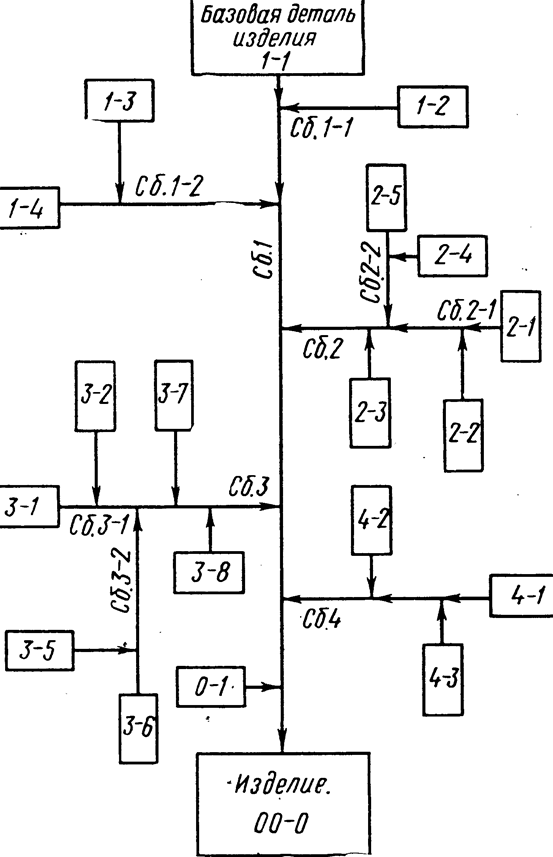
\includegraphics[width=0.6\textwidth]{95_scheme_with_base_component.png}
\caption{Схема сборки с базовой деталью}
\label{fig:95_scheme_with_base_component}
\end{figure}

\subsection*{Схема сборки веерного типа}

Схема сборки «веерного» типа показывает, из каких деталей образуется сборка. Достоинством такой схемы является ее простота и наглядность, но она не отражает последовательность сборки.
Схемами сборки пользуются при разработке технологического процесса наряду со сборочным чертежом и техническими условиями.
Различают стационарную и подвижную сборку.

\begin{figure}[H]
\centering
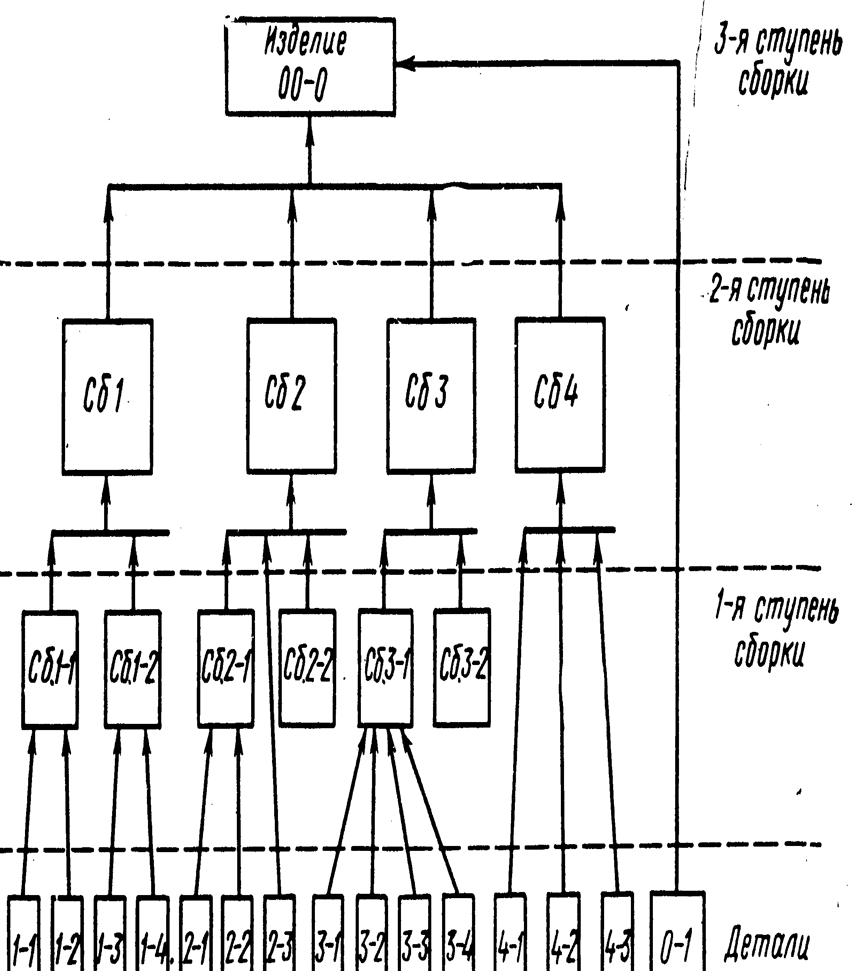
\includegraphics[width=0.6\textwidth]{95_scheme_fan.png}
\caption{Схема сборки веерного типа}
\label{fig:95_scheme_fan}
\end{figure}

\subsection*{Стационарная сборка}

Стационарная сборка выполняется на одном рабочем месте, к которому подаются все необходимые детали и сборочные единицы. Она является наиболее распространенным видом сборки в условиях единичного и серийного производства.

Стационарная сборка может строиться по принципу концентрации и дифференциации. При концентрации весь сборочный процесс выполняется одним сборщиком, а при дифференциации разделяется на предварительную и окончательную. Предварительная сборка производится несколькими отдельными бригадами параллельно, а общая сборка --- специальной бригадой или одним рабочим. Это обеспечивает специализацию рабочих и сокращает длительность сборки.

\subsection*{Подвижная сборка}

Подвижная сборка выполняется при перемещении собираемого изделия от одного сборочного места к другому. На каждом рабочем месте выполняется одна повторяющаяся операция.

Эта форма сборки применяется в условиях поточного производства. Она может осуществляться двумя способами:

\begin{enumerate}
\item со свободным движением собираемых объектов, перемещаемых от одного рабочего места к другому вручную или при помощи механического транспортера;
\item с принудительным движением собираемых объектов, которые перемещаются посредством конвейера при строго рассчитанном такте.
\end{enumerate}

Процесс сборки осуществляется непосредственно на конвейере. Поточная сборка является основной формой, применяемой в серийном и массовом производстве. Переход на поточные методы повышает производительность труда за счет технических и организационных мероприятий, а также сокращает длительность производственного цикла и размер незавершенного производства.

Различия в организационных формах поточного производства сводятся к различиям в поточных линиях (по степени специализации, степени ритмичности, способу поддержания ритма работы, оснащенности транспортными устройствами и др.).


% Вопрос 96 -----------------------------------------------------------------------------
\section{Нормирование затрат времени при проектировании технологических процессов (штучное и подготовительно-заключительное время, определение такта и ритма выпуска изделий).}

Росту производительности труда в значительной степени способствует техническое нормирование --- установление обоснованных норм расхода производственных ресурсов. Под производственными ресурсами понимаются энергия, сырье, материалы, инструмент, рабочее время и т. д.

Техническое нормирование позволяет целесообразно организовать технологический процесс, определить численный и квалификационный состав рабочих, рассчитать количество оборудования и др.

Норма времени --- регламентированное время для выполнения некоторого объема работ в определенных производственных условиях одним или несколькими исполнителями соответствующей квалификации. Норма времени включает в себя штучное время Тш и подготовительно-заключительное время Тп.з.

Штучное время. Составными частями нормы штучного времени являются основное время Т0, вспомогательное время Тв, время обслуживания рабочего места Тобсл, время необходимых перерывов в работе Тпер.

Основное время --- часть штучного времени, затрачиваемая на изменение и (или) последующее определение состояния предмета труда. Основное время может быть машинным, машинно-ручным или ручным.

Вспомогательное время --- часть штучного времени, затрачиваемая на выполнение приемов, необходимых для обеспечения изменения и последующего определения состояния предмета труда. Оно повторяется с каждым обрабатываемым изделием и является преимущественно ручным (установка и снятие обрабатываемых деталей, перестановка инструмента, измерение деталей, управление механизмами станка).

Время обслуживания рабочего места --- часть штучного времени, затрачиваемая исполнителем на поддержание средств технического оснащения в работоспособном состоянии и уход за рабочим местом (подналадка оборудования, смена затупившегося инструмента, удаление стружки и др.).

Время необходимых перерывов в работе --- часть штучного времени, затрачиваемая на личные потребности и дополнительный отдых (при тяжелых работах). Тш = То + Тв + Тобсл + Тпер

Норма штучного времени определяется как сумма его элементов.

Оперативное время --- часть штучного времени, равная сумме основного и вспомогательного времени: Топ = То + Тв. Это время затрачивается на осуществление работы, непосредственным результатом которой является выполнение заданной операции: Тш = Топ + Тобсл + Тпер

Подготовительно-заключительное время. Это время представляет собой интервал времени, затрачиваемый на подготовку исполнителя и средств технологического оснащения к выполнению технологической операции и приведению этих средств в порядок после окончания смены. Оно затрачивается рабочим один раз на выполнение определенной операции (работы) и не зависит от количества п деталей в партии.

Подготовительно-заключительное время входит в норму штучно-калькуляционного времени: Тш.к. = Тш + Тпер / n

Нормы времени устанавливают для каждой операции и типа производства, так как на выполнение одинаковой работы в условиях единичного, серийного и массового производства затрачивается различное время. Основным методом установления норм является расчетно-аналитический. В условиях крупносерийного и массового производства этот метод дополняется исследованием операций непосредственно на рабочих местах, а в мелкосерийном и единичном --- методом сравнения.

Для всех автоматизированных и механизированных операций, выполняемых на металлорежущих станках, аппаратах шовной сварки и другом оборудовании с автоматической подачей, основное время на каждый переход определяется по формуле: $T_0 = L_i / S_M$, где $L$ --- путь, проходимый инструментом или заготовкой в направлении подачи, мм; $S_M$ --- скорость подачи, мм/мин; $i$ --- число проходов.

Вспомогательное время TВ определяется по нормативам, устанавливающим продолжительность отдельных приемов работы. Для сборочных, монтажных, регулировочных, формовочных и других ручных работ обычно определяется оперативное время.

Время обслуживания рабочего места для всех операций, кроме обработочных, исчисляется в процентах (1...7\%) от оперативного времени. Время необходимых перерывов в работе предусматривается в размере 2\% от оперативного времени.

Определение квалификации работы производится по тарифно-квалификационному справочнику. Разряд работы предопределяет наличие признаков, указывающих на подготовку, знания, навыки рабочего и степень его самостоятельности в выполнении работы.

Определяют такт сборки по формуле: Tв = 60F / N (мин/шт), где F --- годовой фонд рабочего времени, час.; N --- годовая программа выпуска, шт.

Если такт значительно превосходит среднюю длительность операции, то сборку ведут по принципу серийного производства, если такт близок или меньше средней длительности операции, то сборку ведут по принципу массового производства.


% Вопрос 97 -----------------------------------------------------------------------------
\section{Изготовление деталей ЭС методом литья.}

Литьем изготавливают отдельные детали несущих конструкций, направляющие, корпуса магнитных головок, приводы накопителей на магнитных дисках и др. Литье --- наиболее простой и дешевый метод формообразования заготовок. Основным инструментом литейного производства является форма. От качества изготовления формы и материала, из которого она изготовлена, зависит качество заготовки (отливки). Формы делятся на разовые, полупостоянные и постоянные. Разовые --- на одну отливку, полупостоянные --- на несколько, постоянные позволяют получить до нескольких тысяч отливок.

\begin{figure}[H]
\centering
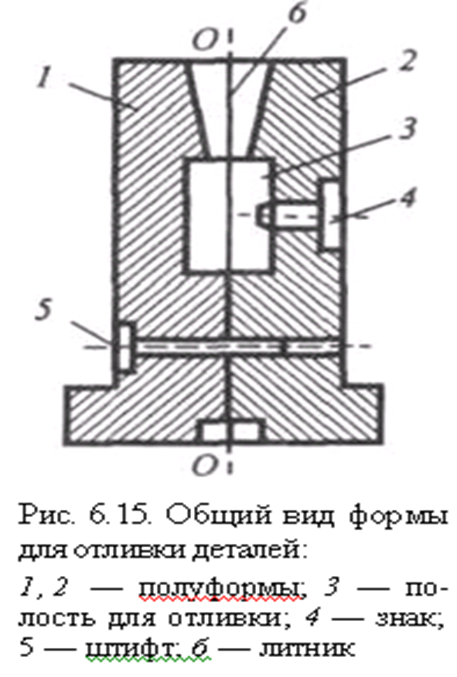
\includegraphics[width=0.3\textwidth]{97_form1.png}
\caption{Литьевая форма}
\label{fig:97_form1}
\end{figure}

Две полуформы 1 и 2 образуют полость 3, в которой образуется отливка. Знак 4 служит для получения углубления в отливке. Штифт 5 центрирует две полуформы при сборке. Отверстие конической формы 6, называемое литником, служит для заливки расплавленного металла в форму. После застывания металла форму разбирают по плоскости разъема О-О, вынимают отливку, затем удаляют литник.

При конструировании литых деталей необходимо учитывать литейные свойства заливаемого металла (сплава): жидкотекучесть, кристаллизацию и усадку. От жидкотекучести во многом зависит минимальная толщина s стенок отливки. Кристаллизация (застывание) сплава происходит в направлении, перпендикулярном поверхности теплоотдачи. Скорость кристаллизации меняется от максимальной у поверхности до минимальной в центре отливки, при этом происходит рост кристаллов к центру.

Усадка --- свойство металлов (и их сплавов) при охлаждении уменьшаться в объеме.

Это необходимо учитывать, обеспечивая отливке плавные переходы от од ной стенки к другой, радиусы скруглений, равностенность и т. п. Если этого не учесть, возможны появления трещин, раковин, перекосов стенок. В производстве ЭС широкое распространение получил способ литья под давлением.

Литье под давлением --- самый производительный и экономичный способ изготовления тонкостенных деталей сложной конфигурации в серийном производстве. Формы изготавливают из металла высокой прочности, с точностью на 2---3 квалитета выше получаемого квалитета у отливки. Получаемая шероховатость отливок составляет 7---8 класс. Наиболее распространено литье под давлением сплавов на основе цинка, алюминия, магния и меди (латуни). В качестве основного оборудования используют литьевые машины, с горячей камерой прессования, с холодной вертикальной и горизонтальной камерой прессования. Тип машины характеризуется устройством прессующего механизма. В настоящее время используют машины с передачей давления на металл посредством поршня. Такие машины называют поршневыми, они бывают с горячей и с холодной камерой прессования.

\begin{figure}[H]
\centering
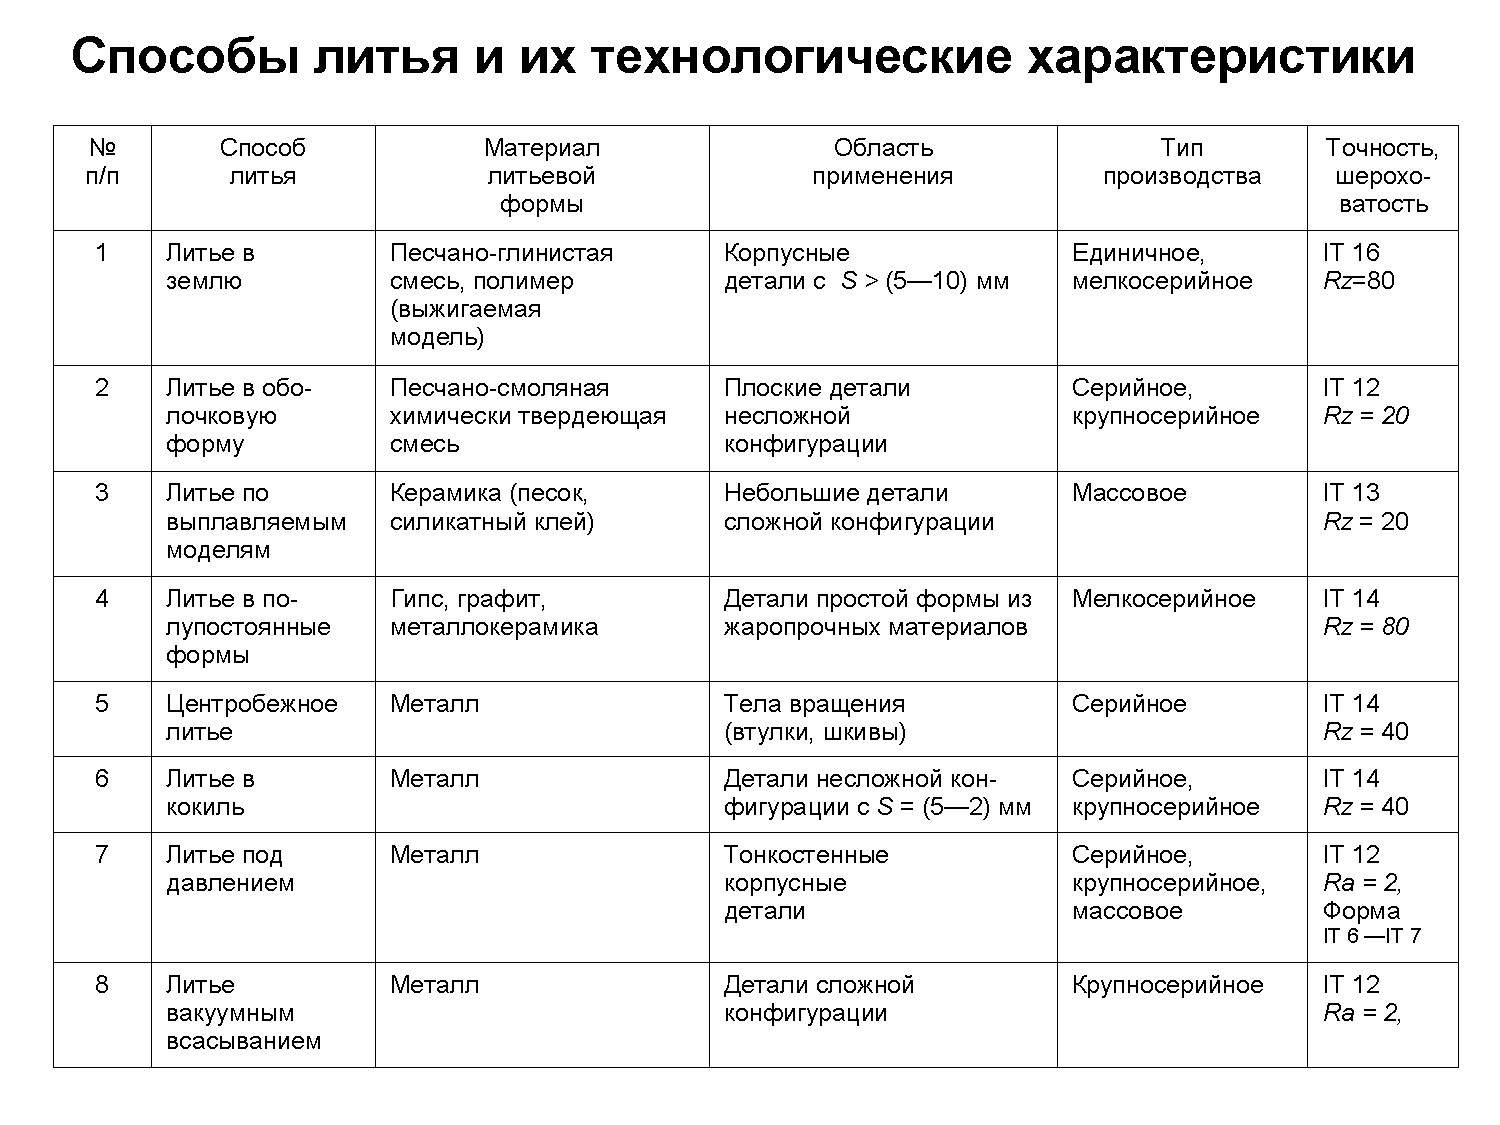
\includegraphics[width=\linewidth]{97_class.pdf}
\end{figure}

Машины с горячей камерой прессования применяют для отливки деталей из цинковых сплавов. Камера прессования таких машин расположена непосредственно в расплавленном металле. Металл из раздаточной печи заливается в подогретый тигель 1. При работе прессующего цилиндра 3 поршень 4 опускается, перекрывает отверстие 8, через которое расплавленный металл поступает в полость камеры 2. Под давлением поршня металл поднимается по каналу 7 и через мундштук 6 заливается в форму 5. Машины с горячей камерой имеют гидравлический или пневматический привод, просты по устройству, высокопроизводительны и могут быть полностью автоматизированы.

После заливки расплавленного металла в камеру прессования 2 поршень 1 опускается и, надавливая на основание 4, открывает литниковое отверстие. Металл заливается в форму 3. Когда он затвердеет, основание 4 поднимается и срезает остаток 5, освобождая выход отливки 6 вместе с литником.

В литьевых машинах с горизонтальной камерой прессования литниковая система более короткая, в таких машинах меньше потери тепла и давления при подаче расплава из камеры прессования в полость формы. Расплавленный металл заливается в горизонтальную камеру через отверстие и под действием поршня запрессовывается в форму. При раскрытии формы остаток металла остается на плоскости разъема. После полного выхода поперечного стержня отливка вместе с литником и остатком выталкивается из подвижной половинки формы.

\begin{figure}[H]
\centering
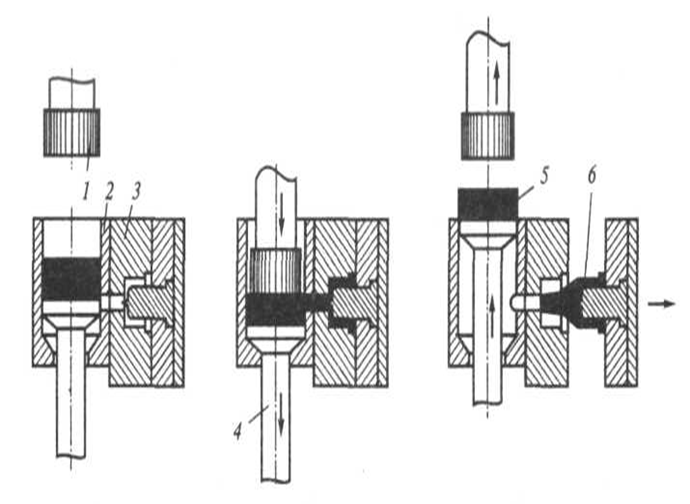
\includegraphics[width=0.7\textwidth]{97_form2.png}
\caption{Схема литьевой машины с холодной вертикальной  камерой прессования: а --- заливка; б --- прессование; в --- раскрытие формы}
\label{fig:97_form2}
\end{figure}


% Вопрос 98 -----------------------------------------------------------------------------
\section{Разделительные и формообразующие операции холодной штамповки.}

Холодная штамповка --- высокопроизводительный, малоотходный довольно точный метод формообразования деталей ЭС. Этим методом изготавливают каркасы, направляющие в каркасах, пластины магнитопроводов, клеммные зажимы и многие другие детали. Исходными материалами для холодной штамповки являются листы, полосы, ленты из черных и цветных металлов, неметаллических материалов (картон, резина, фибра, текстолит. Предварительно исходный материал раскраивают, размещая будущие детали с наименьшими отходами.

\begin{figure}[H]
\centering
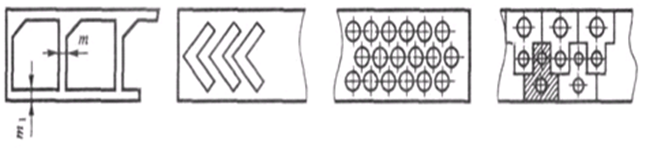
\includegraphics[width=0.7\textwidth]{98_cutting.png}
\caption{Виды раскроя перед штамповкой}
\label{fig:98_cutting}
\end{figure}

На технологичность конструкции штампованных деталей оказывают влияние три основных фактора: ограничения по деформируемости данного материала, допуск на размеры, требования к чистоте поверхности. Первый фактор особенно проявляется при изготовлении сложных полых деталей, требующих большой пластической деформации.

Операции холодной штамповки можно разбить на две основные группы: разделительные и формообразующие. 

К разделительным операциям относятся: отрезка, вырубка, пробивка, надрезка, просечка, зачистка, калибровка; 

К формообразующим --- операции, в результате которых происходит изменение формы и размеров заготовки: гибка, вытяжка, правка (рихтовка), формовка, холодное выдавливание.

\begin{figure}[H]
\centering
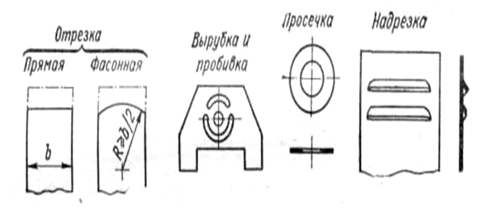
\includegraphics[width=0.6\textwidth]{98_operations.png}
\caption{Виды разделительных операций}
\label{fig:98_operations}
\end{figure}

\begin{figure}[H]
\centering
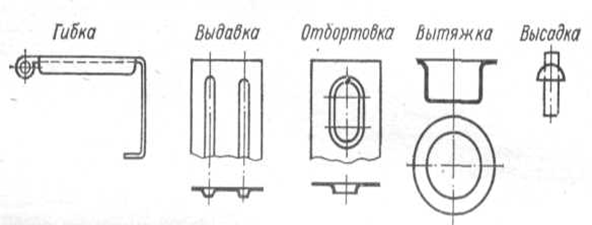
\includegraphics[width=0.7\textwidth]{98_operations2.png}
\caption{Виды разделительных операций}
\label{fig:98_operations2}
\end{figure}

% Вопрос 99 -----------------------------------------------------------------------------
\section{Общая характеристика методов формообразования материалов и деталей при производстве ЭС.}

В конструкции современных ЭС используется большое количество разнообразных металлических и неметаллических деталей, выполняющих различные функции: детали, образующие несущую конструкцию ЭС и обеспечивающие устойчивость их к механическим нагрузкам и климатическим воздействиям; элементы управления, без которых невозможна эксплуатация ЭС; корпусные детали, обеспечивающие эргономические и эстетические характеристики ЭС; детали электромеханических узлов --- накопителей на магнитных дисках, датчиков, печатающих устройств, преобразователей, графопостроителей, сканеров и др. 

К примеру, разберем внешний вид вычислительно-управляющей системы с входящими в нее устройствами, встроенной в базовый несущий каркас. Логично, что данная система состоит из металлических и неметаллических деталей, технологические методы изготовления которых различны и требуют разнообразного технологического оборудования, соответствующей оснастки и приспособлений. К таким методам относятся в первую очередь обработка материалов резанием (механообработка), литье, обработка давлением, электрохимические и электрофизические методы, обработка пластмасс.

Если трудоемкость изготовления ЭС принять за 100\%, то операции механической обработки могут составлять до 15\%, операции литья деталей --- до 3\%, операции обработки давлением --- до 18\%, операции переработки пластмасс --- до 12\%, электрофизические и электрохимические операции --- до 5\%, остальное --- сборка и монтаж. Рассмотрим в общем виде эти методы обработки материалов и формообразования применительно к технологии производства ЭА.

Детали конструкций из металлов и их сплавов получают различными методами формообразования, причем исходный материал может находиться в расплавленном, горячем (раскаленном) или холодном состоянии. Ниже представлена классификация основных методов металлообработки, используемых при изготовлении деталей электронных средств. В классификацию не вошли некоторые специальные, относительно редко применяющиеся виды обработки, такие как электроискровая, электрохимическая, специальные виды литья и т.д.

\begin{figure}[hbtp]
\centering
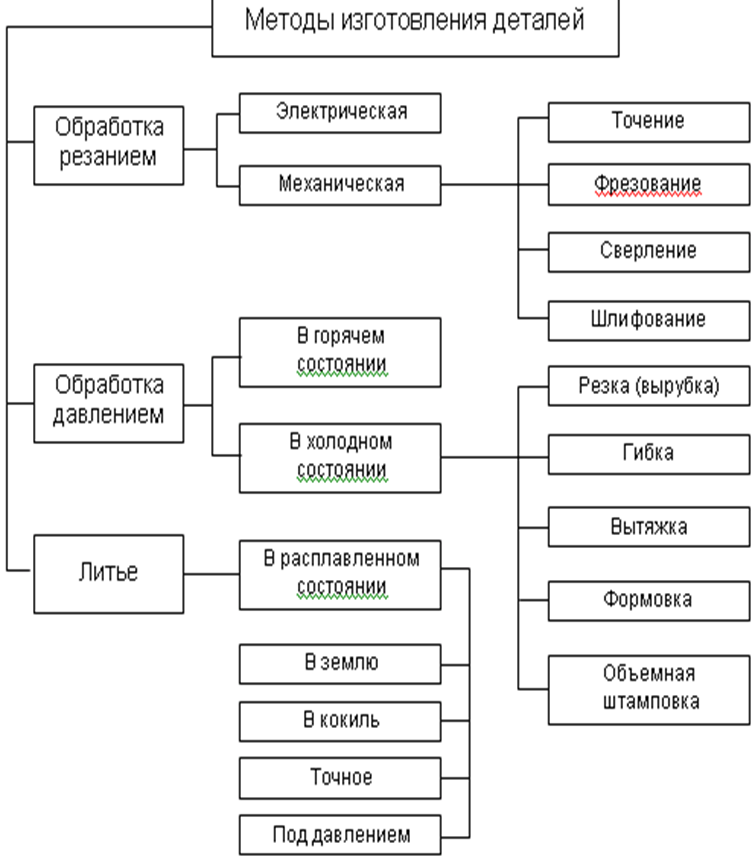
\includegraphics[width=0.8\textwidth]{99_scheme.png}
\caption{Классификация основных методов металлообработки}
\label{fig:99_scheme}
\end{figure}

Использование того или иного вида обработки при изготовлении металлических деталей определяется назначением детали, ее конструкцией, применяемым материалом и другими факторами. Дополнительными факторами являются наличие соответствующего сортамента материала и оборудования на предприятии.. Прогрессивные методы формообразования, такие как штамповка, литье под давлением лишены этих недостатков, однако их применение оправдано лишь при массовом производстве. Это связано с необходимостью проектирования и изготовления дорогостоящей оснастки --- пресс-форм, штампов и т.д.

При изготовлении металлических конструкций приведенные методы изготовления могут комбинироваться как между собой, так и с различными способами соединения деталей (сваркой, склепыванием, склеиванием и т.д.).


% Вопрос 100 ---------------------------------------------------------------------------------------------------------------
\section{Изготовление электронных модулей по технологии внутреннего монтажа.}

Одно из направлений развития электронных модулей, которое по праву относится к российским изобретениям и где мы являемся лидерами --- это технология внутреннего монтажа. Технология внутреннего монтажа устраняет необходимость в корпусировании ИС и производстве многослойных печатных плат. Главное же то, что данная технология придает электронному блоку новые характеристики и устраняет недостатки, присущие технологии поверхностного монтажа. Суть данной технологии сводится к тому, что кристаллы ИС монтируются в специальных углублениях внутри керамических, металлических или полимерных плат с последующим монтажом пассивных и прочих элементов на поверхности печатных плат. Выгоды, которые дает данное направление, представлены в табл.

\begin{figure}[H]
\centering
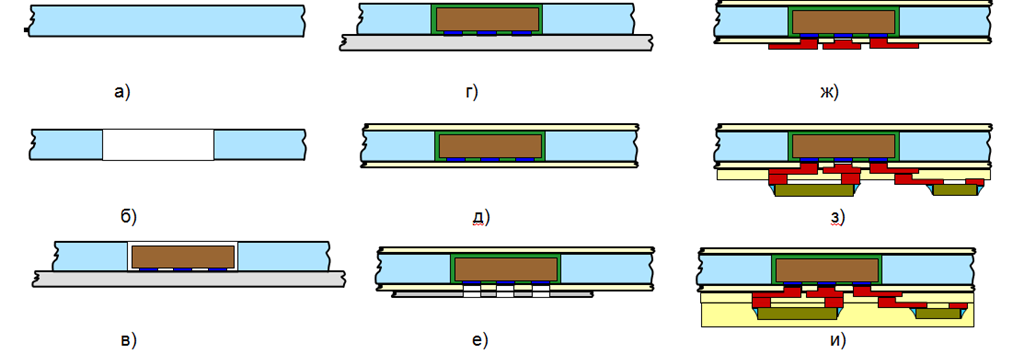
\includegraphics[width=1.0\textwidth]{100_types.png}
\caption{Последовательность операций изготовления радиоэлектронного узла  с внутренним монтажом}
\label{fig:100_types}
\end{figure}

а --- основа печатной платы (металлическая, керамическая, поликоровая); б --- пробивка отверстий для установки кристаллов бескорпусных микросхем; в --- позиционирование кристаллов микросхем в отверстия.; г ---  фиксация кристаллов микросхем компаундом; д --- нанесение защитного диэлектрического париленового (полипараксиленового ) покрытия; е --- ионно-химическое травление через металлическую маску окон над контактными площадками кристалла ИС; ж --- вакуумное осаждение многослойного  (Ti-Cu-Ni) покрытия; з ---  повторение операций д, е, ж (до 30 слоев) и установка пассивных компонентов; и --- окончательная электро- и влагозащита париленовым покрытием

Технология внутреннего монтажа реализуется следующим образом:

\begin{enumerate}
\item на подложке из алюминия штампом пробиваются прямоугольные отверстия соответствующие, с допустимым увеличением, размерам кристаллов ИС, монтируемых в данное отверстие;
\item методом анодирования на подложке формируется диэлектрический слой;
\item подложка укладывается на ровную поверхность монтажного столика, и кристаллы устанавливаются в отверстия активной стороной вниз. Манипулирование кристаллами производится вакуумным захватом, удерживающим кристалл за неактивную сторону кристалла; 
\item заложенные в подложку и планоризированные с нижней стороны подложки кристаллы фиксируются в ней компаундом, наносимым в зазор между кристаллом и подложкой;
\item после полимеризации компаунда подложка с кристаллами помещается в установку нанесения париленового (полипараксилиленового) покрытия, где при температуре 28\textcelsius на поверхности подложки и лицевых сторонах кристаллов происходит формирование диэлектрического слоя --- париленовой пленки; 
\item через металлические маски в слое парилена ионно-химическим травлением вскрываются окна над контактными площадками ИС. Одновременно происходит очистка контактных площадок перед напылением проводников; 
\item в установках вакуумного напыления через свободные технологические маски производится напыление проводников Ti --- Cu --- Ni.
Указанные операции осаждения слоя парилена, вскрытия окон, вакуумной металлизации могут повторяться необходимое количество раз для формирования нужного количества слоев (до 30 слоев), причем переход со слоя на слой производится с помощью отверстий, диаметр которых не превышает ширину проводника;
\item пассивные элементы функционального электронного блока припаиваются к печатной плате традиционными способами, как элементы поверхностного или штырькового монтажа;
\item окончательная электро- и влагозащита обеспечивается внешним париленовым покрытием.
\end{enumerate}
Приведенная технология применима как при корпусировании ИС, так и при непосредственном монтаже кристаллов внутри функционального электронного блока. Тепловая разгрузка кристаллов смонтированных вышеприведенным способом, обеспечивается как напылением слоя металла на заднюю поверхность кристалла и подложки в целом, так и напылением слоя металла на тонкий слой диэлектрика с лицевой стороны кристалла и печатной платы. Кроме того плата с кристаллами может быть плотно присоединена к дополнительным теплоотводящим основаниям --- радиаторам. На поверхности теплоотвода могут быть сформированы дополнительные слои коммутации с использованием полимидных пленок с вакуумной металлизацией.
Для реализации метода необходимы в основном два вида оборудования:

\begin{itemize}
\item установки вакуумного напыления;
\item установки ионного травления.
\end{itemize}

Помимо увеличения плотности монтажа в несколько раз благодаря отсутствию выводов микросхем, уменьшения ширины проводников до 50 --- 70 мкм, снижению диаметра переходного отверстия до 25 --- 30 мкм, также увеличивается надежность за счет следующего:

\begin{itemize}
\item отсутствие сварных и паяных контактов;
\item проводник формируется сухим методом и состоит из чистых материалов, не содержит никаких остатков травления, являющихся фактором деградации тонких проводников обычных печатных плат;
\item близость коэффициентов линейного расширения кристалла, оксидного защитного слоя подложки, керамических корпусов конденсаторов и ситалловых корпусов резисторов для поверхностного монтажа обеспечивает безотказную работу блоков при резких перепадах температуры;
\item кристаллы ИС, уложенные в алюминиевую или керамическую подложку, находятся в условиях постоянной теплоразгрузки на тело подложки, что создает надежные условия эксплуатации ИС.
\item подложка из алюминия естественным образом создает не только теплоразгрузку кристаллов, но и обеспечивает защиту схемы от постороннего электромагнитного воздействия.
\end{itemize}

\begin{figure}[H]
\centering
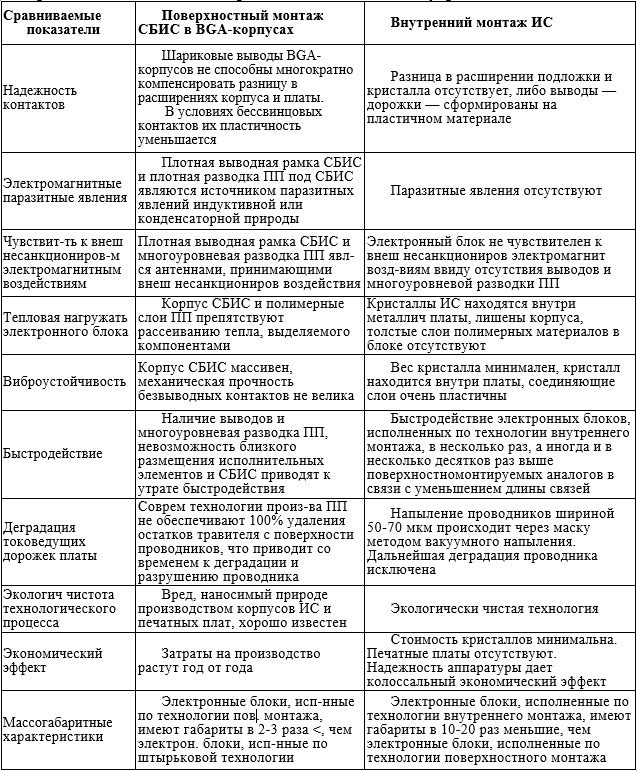
\includegraphics[width=0.8\textwidth]{100_table.png}
%\caption{Последовательность операций изготовления радиоэлектронного узла  с внутренним монтажом}
%\label{fig:100_table}
\end{figure}

\end{document}